\chapter{Äriplaan}
\section{Arendus- ja halduskuludest}
\label{sec:kulud}
Laias laastus võib öelda, et kulud arendusele jagunevad kuludeks\index{Kulud!Arendus}index{Kulud!Haldus}, mis tarnivad uut funktsionaalsust (ning mida tavaliselt tajutakse kui uut väärtust\index{Väärtus} lisavatena) ning kuludeks, mis lähevad olemasoleva muutmiseks või parandamiseks. Neist esimesed lisavad selgesti halduskoormust ja halduskulusid luues uusi rakendusi, mida tuleb hallata, millede teenustase tuleb tagada. Teised aga võivad (aga ei pruugi) halduskulusid vähendada näiteks tehnilist tehnilist võlga likvideerides. Arenduskulusid võib vaadata ka keerukuse vaatepunktist: esimest liiki kulud suurendavad, teised võivad aga keerukust vähendada. Kokkuvõte kuludest ja nende mõjudest on toodud tabelis \ref{tab:arendus}.

\begin{table}
	\begin{center}
		\begin{tabular}{p{2.8cm}p{1.7cm}p{1.5cm}p{2cm}}
		\toprule
Kulu & Mõju haldus\-kuludele & Mõju tajutud väärtusele & Mõju \mbox{keerukusele} \\
\midrule

Uue funktsionaaluse \mbox{lisamine} & Selgesti \mbox{suurendab} & Selgesti \mbox{suurendab} & Selgesti \mbox{suurendab} \\
\addlinespace
Olemasoleva muutmine või parandamine & Neutraalne või vähendab & Reeglina \mbox{neutraalne} & Neutraalne, \mbox{pigem} vähendab \\

\bottomrule
		\end{tabular}
		\caption{Kokkuvõte arenduskulude mõjust}
		\label{tab:arendus}
	\end{center}
\end{table}

Siit tuleneb oluline tõdemus: arenduskulud, mis suurendavad tajutud väärtust tekitavad juurde ka halduskoormust ja lisavad keerukust viies seega alla organisatsiooni võime tulevikus uut väärtust lisada. Võtmeks tupikust välja on sõna "tajutud". Muutes viisi, kuidas organisatsioon tajub ITst tulenevat väärtust on võiamlik saavutada tellija arusaam IT kulude dünaamikast.

Nagu kõik investeeringud, on investeeringud ITsse finantsjuhtimise objektiks. Investeeringud amortiseeritakse teatud perioodi  jooksul ja kulud kaetakse jooksvast eelarvest. Kui äriorganisatsioonil on fikseeritud aastane kulueelarve IT suunas, tekib kiusatud suuremahulised projektid teha investeeringutena ning hiljem katta vaid amortisatsioonikulusid. Selline lähenemine tuleneb kogemusest materiaalse põhivaraga, kus põhivara haldamiseks tehtavad kulutused on oluliselt väiksemad amortisatsioonikuludest. Investeerides näiteks mõnda masinasse, see kulub kuni ei ole enam mõistlikult kasutatav. Jah, igakuiselt tuleb maksta hooldusarveid, kuid need on tüüpiliselt oluliselt väiksemad, kui liisingmakse. Samuti on hoolduskulud tavaliselt äriplaanis juba toote omahinnana arvesse võetud. 

Infosüsteemide puhul on olukord oluliselt erinev. Pärast algset investeeringut tarkvara loomisse, hakkavad jooksvalt tekkima vähemalt järgmised kulud:
\begin{description}
	\item[Serverid, võrguseadmed ja nende majutus] Serverid amortiseeruvad, neid peab hoidma jahedas valvatavas ruumis ning nad võtavad elektrit
	\item[Süsteemi monitooring] Keerukad infosüsteemid vajavad tüüpiliselt mingit jälgimist, halvemal juhul 24/7. 
	\item[Klienditugi] Reeglina vajab infosüsteem teatud tuge kliendile. Olgu selleks õiguste lisamine ja eemaldamine, finantsaasta vahetusega seotud tegevused, tavapärane tõrkeotsing või lihtne kliendi õpetamine, peab leiduma keegi, kes vajadusel süsteemi kapoti alla vaatab
	\item[Internetiühendus] Infosüsteemi kasutatakse reeglina läbi internetiühenduse. Korralik internetiühendus maksab raha ning see kulu ei pruugi olla väike. Keerukamatel juhtudel lisanduvad veel kulud CDNile\sidenote{CDN - \emph{Content Delivery Network}. Süsteem, mis vähendab kasutaja poolt tajutud latentsi tehes süsteemi osad kättesaadavaks lõppkasutajale interneti topoloogia mõttes soodsates asukohtades} ja muule sellisele
	\item[Turvateenused ja riistvara] Infosüsteemid vajavad kaitset ning vastavat riist- ja tarkvara ning teenuseid on turul saadaval. Turvaseadmed on näiteks tulemüürid ja riistvaralised SSL-kiirendid ning teenusena võib sisse osta kõike alates operatsioonisüsteemi paikamisest kuni teenustõrkerünnete vastasest taristust  
	\item[Infoturve] Lisaks riistvarale ja tarkvarale vajab iga infosüsteem pidevalt infotehnoloogilist tähelepanu. Küberruumis kasutatavad ründevahendid arenevad pidevalt ning nii teie loodud tarkvaras kui seda toetavates süsteemides tuvastatakse pidevalt turvavigu. Nende vigade järgimine ning tarkvara uuendamine vajavad küllalt spetsiifilist kompetentsti.
\end{description}

Kõigil neil kuludel on kolm omadust:
\begin{enumerate}
	\item Nad on üksteisest raskesti konkreetsele süsteemile allkoeeritavad. Kui organisatsioonil juba on 24/7 monitooringuvõimekus, eeldab see hulka hästi organiseeritud inimesi. On üsna keeruline hinnata, kui palju tööd lisab neile iga konkreetne uus lahendus. Inimene on öösel telefonivalves ju igal juhul? Kui suure osa serveriruumi külmast õhust võtavad just konkreetse süsteemi serverid?
	\item Nad on arenduskulude\sidenote{Mis omakorda genereerivad halduskulusid käivitades omaette tagasiside} kaudu tagasisidestatud. Monitooring ja klienditugi võivad avastada süsteemist parandamist vajava vea, infoturve võib leida, et süsteemi riskide aktsepteerivale tasemele viimiseks on vaja teha arendustööd. Süsteemi piisava jõudluse tagamiseks ei pruugi olla võimalik enam riistvara lisada. Kõik muutused tarkvaras aga tekitavad uusi vigu, vajadust klienti toetada, jõnkse monitooringule, tegevust infoturbele jne. 
\end{enumerate}

Kõik need kulud moodustavad tüüpiliselt oluliselt suurema ning raskemini hinnatava\sidenote{Siit tuleb üks olulisi pilveteenuste\index{Pilveteenused} võlusid. Kuna need võimaldavad ressursikasutust täpselt hinnata, on nende abil võimalik süsteemide kulutatavat oluliselt selgemini eristada. Kasu tuleb nii privaat- kui avaliku pilve puhul.} protsendi algsest investeeringust, kui materiaalse põhivara puhul. 

Kui pildile lisada veel asjaolu, et tehnoloogia kipub ajas vananema suurendades halduskulusid\sidenote{Vt. \nameref{sec:rooste}}, siis ei ole üldse selge, milline mõju saab olema arendusprojekti amortiseerimisel (hoides kulubaasi stabiilsena kuid vähendades kulusid jooksvale haldusele ning arendusele) või kohe kulusse kandmisel.

Küsimus arenduskulude juhtimisest on eriti oluline avalikus sektoris. Ühest küljest puudub siin kasumlikkuse surve\sidenote{18f, USA föderaalvalitsuse digitaalagentuuri blog on hea allikas avaliku sektori it-probleeme lahkavate artiklite osas. \url{https://18f.gsa.gov/2016/02/23/software-maintenance-is-an-anti-pattern/} on selle lõigu inspiratsiooniks} ja teisalt on kulud ja investeeringud reeglina rangelt eraldatud. Mõlemad seavad süsteemi hooldamiseks tehtavad kulutused tugeva surve alla: esimene tekitab tunde, et hoolduskulud on ebavajalikud ja teine võimaldab taotleda finantseeringut projektidele, mille hooldamiseks puuduvad vahendid. Nii tekib olukord, kus oluline investeering ei tooda puuduva hoolitsuse tõttu maksumaksjale piisavalt väärtust. 

Probleemi ületamiseks pakub 18f, et igal süsteemil peaks käivitusperioodi lõppedes tekkima eri osapoolte esindajatest (sh. arendajad) koosnev meeskond, mis tegeleb järgmisega
\begin{description}
	\item[Kasutaja vajadus] Kes süsteemi kasutab? Kas kasutajate rühm kattub algse sihtrühmaga? Kui ei, siis kuidas kasutajad oma vajadusi rahuldavad?
	\item[Konkuretsianalüüs] Millised meie omale sarnased süsteemid turul eksisteerivad ning kas me peaksime neid täiendama (ehk, katma funktsionaalsust, mida nemad ei kata), asendama (pakkuma paremat kvaliteeti ja rohkem funktsionaalsust) või kasutama (sulgema oma teenuse ning ostma selle sisse)
	\item[Kasutatavustestid] Kuidas olemasolevad kasutajad meie süsteemi kasutades käituvad, milline on üldine kasutajakogemus ning kas seda saab parandada?
	\item[Arendussaba sugemine]\sidenote{\enquote{Arendussaba} on maakeelne vaste ingliskeelsele terminile \enquote{Backlog}. Mis oma olemuselt on süsteemi teadaolevate defektide, probleemide ja arendussoovide nimekiri. Mida, on ütlematagi selge, on mõistlik pidada ning aegajalt puhastada, ehk sugeda, eemaldades sealt aegunu ning ebavajaliku.}\index{Arendussaba} Millised read nimekirjas on ühe (millise?) probleemi sümptomid? Millised probleemid suudame olemasolevate vahendite raames parandada ja millised mitte?
	\item[Meetrikate järgimine] Kas NPS\index{Net Promoter Score}\sidenote{\emph{NPS - Net Promoter Score} on kõige lihtsamas versioonis kasutajate keskmine vastus küsimusele \enquote{Kui tõenäoliselt soovitaksid käesolevat teenust sõbrale või kolleegile?}} või mõne muu meetrika väärtus vastab meie ootustele, soovidele ja vajadustele?
\end{description}

\section{Arhitektuur ja äri}
Toote või teenuse arhitektuur mõjutab otseselt orgranisatsiooni ärilist positsiooni. Crawley järgi on igal süsteemil kolm olulist aspekti: vorm, funktsioon ja kontseptsioon (vt. \nameref{sec:arch:fcc}).

Toote või teenuse väärtus tuleneb tema funktsioonist: mida täpsemalt vajadust täidetakse ning mida põletavam too vajadus, seda väärtuslikum toode või teenus. Süsteemiga seotud kulud tulenevad aga kogu elutsükli jooksul vormist: vormi loomiseks tuleb hankida materialid, viia läbi tootmine ning lõpuks utiliseerimine. Järelikult tuleneb vormi ja funktsiooni vahekorrast (mida suuresti määratleb kontseptsioon), süsteemi võimekus väärtust lisada. 

\begin{marginfigure}
	\begin{center}
		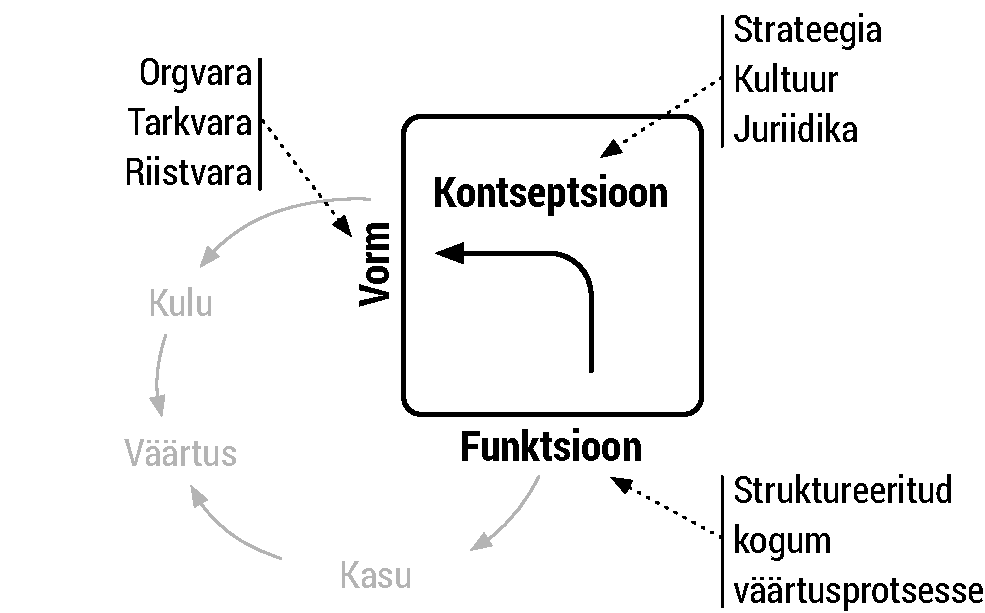
\includegraphics[width=\linewidth]{ffc_profit.pdf}
		\caption{Organisatsiooni eri aspektide seosed omavahel ja organnisatsioon majanduseduga}
		\label{fig:arh}
	\end{center}
\end{marginfigure}

Toote või teenuse võimest väärtust lisada tuleneb aga organisatsiooni kui terviku väärtuse lisamise võime ning seega ka majanduslik jätkusuutlikkus. 

Kasumi ja arhitektuuri seoseid illustreerivaid näiteid on nii kaugemast kui lähemast minevikust mitmeid. Positiivsena tasub esile tuua Black \& Deckeri strateegilist tooteinnovatsiooni seitsmekümnendatel ning Volkswageni platvormistrateegiat. Negatiivsena on üks tuntumaid General Motorsi lähenemine platvormidele. 


\section{Ettevõtte arhitektuurist}
Traditsioonilised EA\footnote{ingl. \emph{Enterprise Architecture}}\index{EA} raamistikud räägivad palju äriarhitektuurist kuid teevad seda abstraktselt. Detailidesse minnakse reeglina vaid infosüsteemide puhul. Paremal juhul eeldadatakse, et muude organisatsiooni aspektide juhtimine võtab üle IT terminoloogia, lähenemise ja mõtteviisi. Organisatsioon koosneb aga liiga paljudest eri taustaga inimeste eri fookusega vastutusaladest, et oleks lootust neile kõigile üht metoodikat rakendada.  Seetõttu on EA kui distsipliin end sageli diskrediteerinud jäädes kageks nii ärist (kes lihtsalt mõtlevad oma probleemidest teisel viisil) kui inseneridest (kes peavad igapäevaselt tegelema ärilise keerukuse valamisega infosüsteemidesse). \sidenote{Vaata ka \nameref{sec:architecture:paradigm}}

Mida siis teha? Soovitusi annab \cite{fowlerlean}. Artiklis on oluline alltekst: kuigi räägitakse arhitekti rollist agiilses organisatsioonis, isegi ei mainita võimalust, et organisatsioon agiilseks \emph{ei muutuks}. Arhitekti roll kaasaegses organisatsioonis peab muutuma. Otsuste tegijast otsuste toetajaks. Suuna andjast sildade ehitajaks. Õpetajast õppiva kogukonna keskmeks. 

\section{Küsimusi aruteluks}
\subsection{Kuidas seletada kliendile, et tema eilsel otsusel on mõju tema tänasele kulubaasile?}
\label{sec:business:q1}
Inimesed, tundub, ei suuda hästi siduda põhjust ja tagajärge. Kindlasti on üheks põhjuseks meie vajadus säilitada positiivset minapilti (\enquote{Ma olen ülekaalus, kuna mu geneetika on selline, mitte seepärast, et ma ei suuda end söömisel ohjeldada}) kuid tõenäoliselt ka evolutsioonilised faktorid. Meid ümbritsev maailm on äärmiselt mittelineaarne ning põhjuse seos tagajärjega muutub aja möödudes järjest ebaselgemaks. 

Kuidas ka ei oleks, inimeste esimene järeldus probleemi põhjuste osas ei ole reeglina endogeenne. Kuigi teooria näitab, et probleemid on harva eksogeensed. 

Ehk, kliendi käitumine ei ole mitte puuduliku personalipoliitika või isikliku küündimatuse tulemus vaid inimesed üldiselt nii käituvadki. Siinkohal olekski lihtne panna punkt, lugeda kogu probleem inimloomuse tõttu lahendamatuks. Siiski on organisatsioon tervikuna keeruline dünaamiline süsteem mille emergentse käitumisena kliendi lühiajalist fookust ka seletada saab. 

\begin{marginfigure}
	\begin{center}
		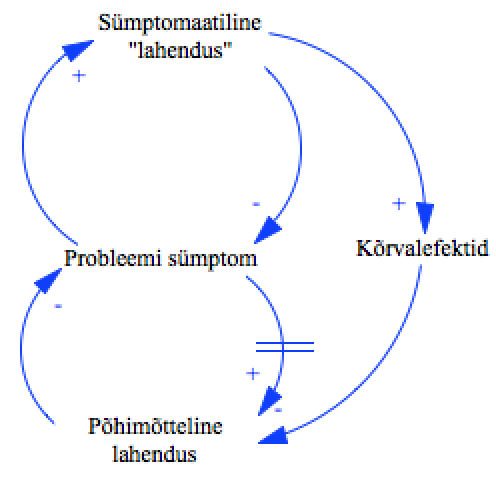
\includegraphics[width=\linewidth]{shiftingburden.png}
		\caption{Koorma nihutamise arhtetüüp.}
		Allikas: Peter Senge
		\label{fig:shifting}
	\end{center}
\end{marginfigure}

Juba viidatud Peter Senge kirjeldab oma raamatus\cite{senge19905th} tervert rida süsteemiarhetüüpe, mis kirjeldavad ettevõtetes ette tulevaid tüüp-probleeme. Üks neist on \enquote{koorma nihutamine}. Juurprobleemiga tegelemise asemel tegeletakse sümptomitega, kuni võimekus päris probleemiga tegeleda või seda isegi ära tunda kaob. Selline käitumine tõesti tihti klienti ka iseloomustab. Kuna juurprobleem (infosüsteemi kõrge hoodlusvajadus elutsükli käigus) ei ole lihtsasti lahendatav, tegeletakse üha uue funktsionaalsuse tellimisega (mis läheb ajas seda kallimaks, mida halvemini hooldatud meie infosüsteem on) kuni kogu kupatus kuulutatakse hallatamatuks, asendatakse uuega ning tsükkel algab otsast.

Senge ütleb, et sellisel puhul ei ole muud väljapääsu, kui tuumprobleemile silma vaatamine. Äriplaanid on liiga optimistlikud (sest jooksvad kulud on nende keerulise struktuuri tõttu raskesti hinnatavad ja ebameeldivalt suured) ja organisatsiooni kulujuhtimine ebapiisav (sest paljud materiaalse põhivara puhul toimivad skeemid immateriaalse puhul hästi ei toimi). Infosüsteem on pigem loom, kelle eest sa taltsutamise järel vastutad, mitte oma amortisatsiooni lõpu poole tiksuv masin.